\documentclass{article}
\usepackage{xcolor}
\usepackage{titleps}
\usepackage[letterpaper, margin=0.95in]{geometry}
\usepackage{url}
\usepackage{amsmath}
\usepackage{amssymb}
\usepackage{wrapfig}
\usepackage{float}
\usepackage{mathtools}
\usepackage{enumitem}
\usepackage{tabu}
\usepackage{parskip}
\usepackage{natbib}
\usepackage{listings}

\usepackage[many]{tcolorbox}
\usepackage{minted}
\setminted[python]{
	% frame=single,
	% linenos,
    xleftmargin=0.475em,
    baselinestretch=1.2,
}
% https://tex.stackexchange.com/a/569249
\setcounter{secnumdepth}{5}
\setcounter{tocdepth}{5}
\makeatletter
\newcommand\subsubsubsection{\@startsection{paragraph}{4}{\z@}{-2.5ex\@plus -1ex \@minus -.25ex}{1.25ex \@plus .25ex}{\normalfont\normalsize\bfseries}}
\newcommand\subsubsubsubsection{\@startsection{subparagraph}{5}{\z@}{-2.5ex\@plus -1ex \@minus -.25ex}{1.25ex \@plus .25ex}{\normalfont\normalsize\bfseries}}
\makeatother

\usepackage{hyperref}
\usepackage[color=red]{todonotes}
\usepackage{forest}
\definecolor{light-yellow}{HTML}{FFE5CC}

\newpagestyle{ruled}
{\sethead{CMU 16-831}{Introduction to Robot Learning }{Fall 2026}\headrule
  \setfoot{}{}{}}
\pagestyle{ruled}

\renewcommand\makeheadrule{\color{black}\rule[-.75\baselineskip]{\linewidth}{0.4pt}}
\renewcommand*\footnoterule{}

\newtcolorbox[]{answer}[1][]{
    % breakable,
    enhanced,
    nobeforeafter,
    colback=white,
    title=Your Answer,
    sidebyside align=top,
    box align=top,
    #1
}



\begin{document}

\lstset{basicstyle = \ttfamily,columns=fullflexible,
backgroundcolor = \color{light-yellow}
}

\begin{centering}
    {\Large Assignment 3: Q-Learning and Actor-Critic Algorithms
} \\
    \vspace{.25cm}
\end{centering}
\vspace{0.25cm}

\textbf{Andrew ID:} \texttt{vawale} \\
\textbf{Collaborators:} \texttt{None. Claude (Anthropic) helped with the code and the text format.}\\ 
\textbf{NOTE:} Please do \textbf{NOT} change the sizes of the answer blocks or plots.

\setcounter{section}{0}
\section{Question 1: DQN and DDQN (LunarLander-v3) - [7.5 points]}
\begin{answer}[title=Question 1,height=9.5cm,width=\linewidth]
\centering
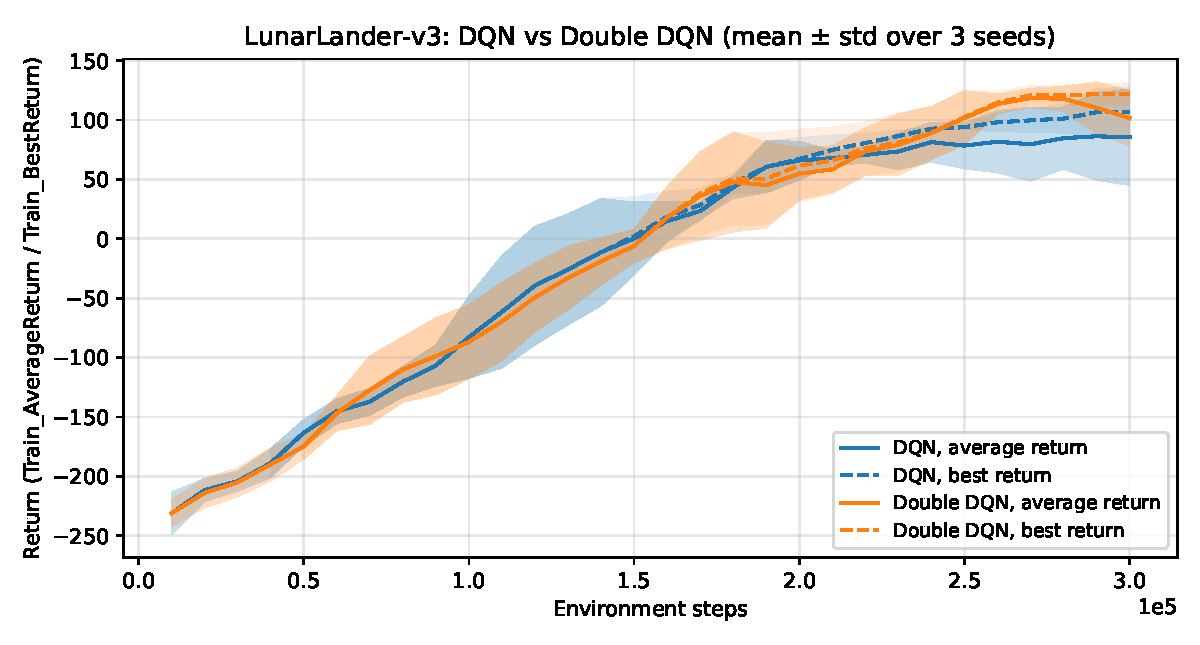
\includegraphics[height=8cm]{figures/q1_dqn_vs_ddqn.pdf}
\end{answer}

\textbf{Figure:} The lines show the mean of seeds 1, 2 and 3. The shaded areas show one standard deviation. The solid lines show \texttt{Train\_AverageReturn}, which is the mean return of the last 100 episodes. The dashed lines show \texttt{Train\_BestReturn}, which is the highest \texttt{Train\_AverageReturn} until that step. All runs use the default hyperparameters from the assignment. All commands include \texttt{--no\_gpu}.

\textbf{DQN and double DQN.} Until $2\times10^5$ steps, the returns of DQN and double DQN increase at the same rate. After $2\times10^5$ steps, the return of double DQN continues to increase, but the return of DQN stays almost constant. At the last step, the mean best return is 122 for double DQN and 107 for DQN. The reference value in the assignment is approximately 125. The mean final average return is 102 for double DQN and 85 for DQN. At the end, the three DQN seeds have larger differences, and one DQN seed decreases from a best return of 92 to 37.

The overestimation of Q-values is the probable cause of this difference. DQN uses the target network to select the next action and also to calculate the value of that action. Because the Q-values contain errors, the $\max$ operation usually selects an action with a value that is too high. With $\gamma = 1$, the bootstrapped target adds this error at each step. Double DQN selects the action with the online network and calculates its value with the target network. This change removes most of the error and gives more stable targets near the end of the run.

There are only three seeds for each method, and the shaded areas overlap. Also, the average return of double DQN decreases slightly in the last evaluations. The data agrees with the expected effect, but it does not give an accurate measurement of the size of the effect.

\section{Question 2: Actor-Critic (CartPole-v0) - [3.75 points]}
\begin{answer}[title=Question 2,height=9.5cm,width=\linewidth]
\centering
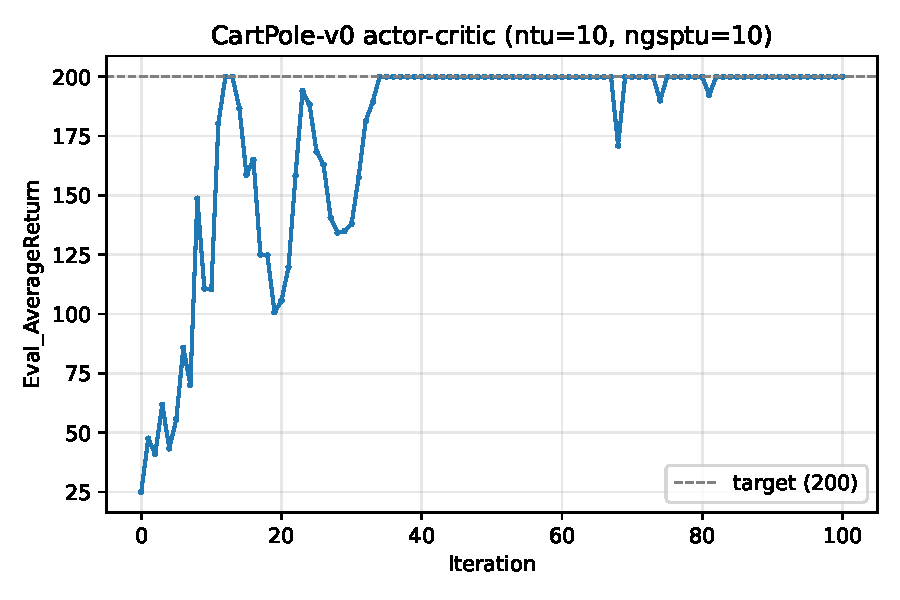
\includegraphics[height=8cm]{figures/q2_cartpole.pdf}
\end{answer}



\section{Question 3: Actor-Critic (InvertedPendulum-v4) - [3.75 points]}
\begin{answer}[title=Question 3,height=9.5cm,width=\linewidth]
\centering
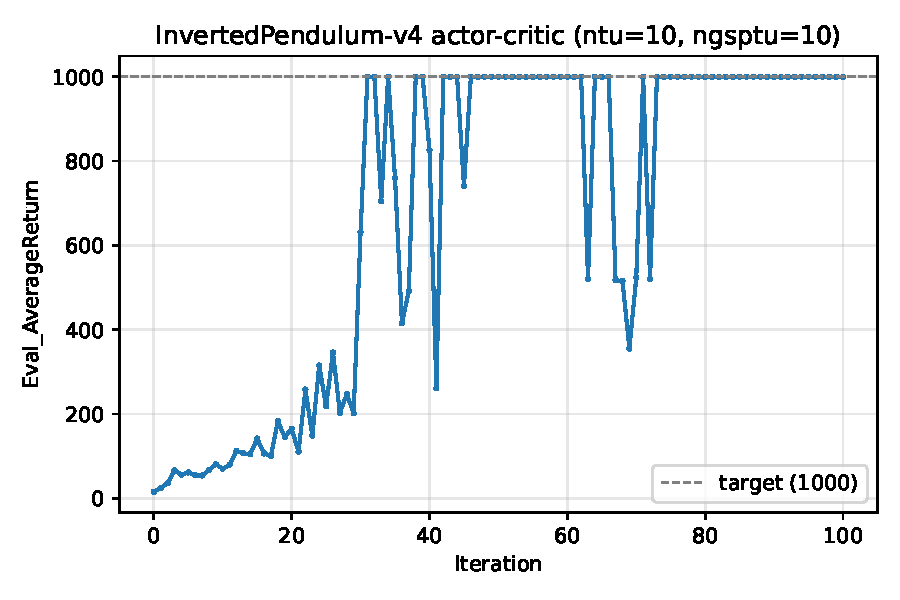
\includegraphics[height=8cm]{figures/q3_pendulum.pdf}
\end{answer}







\end{document}